\documentclass[12pt]{article}
\usepackage{fullpage}
\usepackage{lastpage}
\usepackage{fancyhdr}
\pagestyle{fancy}

\addtolength{\topmargin}{-0.25in}
\usepackage{graphicx}	
\usepackage{array, multicol}
\usepackage{amsmath}
\usepackage{comment}
\usepackage{enumerate}

\everymath{\displaystyle}

\fancypagestyle{plain}{
	\fancyhf{}
	\addtolength{\headheight}{2.92\baselineskip}
	\lhead{\bf MATH 2554 (Calculus I) \\
		Summer 2015 \\
		}
	\rhead{{Name:} \underline{\hspace{40ex}} \\
		\vspace{0.5pc}
		Fri 5 June 2015}
	\rfoot{Exam 1B p.\thepage\ (of \pageref{LastPage})}
	}
\fancyhf{}
\renewcommand{\headrulewidth}{0pt}

\title{\vspace{-8pc}
\vfill{\Huge
	\bf Exam 1: Limits ($\textstyle\oint$2.1-3.1)} \\
	Version B}
\author{}
\date{}

\rfoot{Exam 1B p.\thepage\ (of \pageref{LastPage})}

% % % % %
\begin{document}
\maketitle
\vspace{-3pc}
\noindent{\bf Exam Instructions:} You have 50 minutes to complete this exam.  Justification is required for all problems. 

\vspace{2pc}
\noindent\textbf{Your signature below indicates that you have read this page and agree to follow the Academic Honesty Policies of the University of Arkansas.}  

\vfill
\noindent Signature: {\bf (1 pt)} \underline{\hspace{73ex}}
\begin{flushright}\Large Good luck!\end{flushright}
\begin{enumerate}

% % % % %
\newpage
\item {\bf (14 pts)} Given %$f(x)=2x^3+x$, use the Intermediate Value Theorem to show there exists
$f(x)=x^3-5x^2+2x$, use the Intermediate Value Theorem to show there exists
a solution to the equation %$f(x)=2$ on the interval $(-1,1)$. 
$f(x)=-1$ on the interval $(-1,5)$.
\vspace{22pc}

% % % 
\item {\bf (24 pts)} Determine the end behavior of %$f(x)=\frac{4x^3+1}{2x^3+\sqrt{16x^6+1}}$.
	%\vspace{22pc}
	$f(x)=\frac{4x^3}{2x^3+\sqrt{9x^6+a5x^4}}$.
	\vspace{22pc}
	%$f(x)=2x^{-8}+4x^3$
	%\vspace{22pc}
	%$f(x)=2x^{-8}+3x^4$
	%\vspace{22pc}

% % % % %
\newpage
\item {\bf (5 pts ea)} Evaluate the following limits analytically:
\begin{enumerate}
	%\item $\lim_{t\to 3}\sqrt[3]{t^2-10}$
	%\vspace{14pc}
	\item $\lim_{t\to 2}\,(t^2-t)^5$
	\vspace{14pc}
	%\item$\lim_{\theta\to -\infty}\frac{\cos{(\theta^5)}}{\theta}$
	%\vspace{14pc}
	\item $\lim_{\theta\to\infty}\frac{\cos{\theta}}{\theta^2}$
	\vspace{14pc}
		
	\item $\lim_{x\to -b}\frac{(x+b)^7+(x+b)^{10}}{4(x+b)}$
	\vspace{14pc}
\end{enumerate}

% % % % %
\newpage
\begin{comment}
\item \begin{enumerate}\vspace{-2pc}
	\item {\bf (7 pts)} Using the graph below, find the $\delta$ that satisfies $|f(x)-5|<1$ whenever $0<|x-4|<\delta$.
	\vspace{4pc}
	
	\item {\bf (7 pts)} Use the same graph to find the $\delta$ that satisfies $|f(x)-5|<\textstyle\frac{1}{2}$ whenever $0<|x-4|<\delta$.
	\vspace{4pc}
	
	\item {\bf Extra Credit (4 pts)} Using smaller and smaller $\epsilon$s and finding the corresponding $\delta$s, as in (a) and (b), will show 
	\[\lim_{x\to ?}f(x)=?.\]
	(rewrite the limit, with the ?s filled in).
	\vspace{6pc}
	\end{enumerate}  
\begin{center}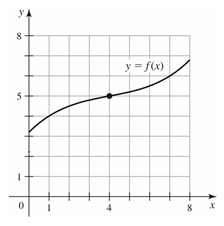
\includegraphics[scale=1.5]{exam1sec2p7}\end{center}
\end{comment}
%\begin{comment}
\item \begin{enumerate}\vspace{-2pc}
	\item {\bf (7 pts)} Using the graph, find the $\delta$ that satisfies $|f(x)-6|<3$ whenever $0<|x-3|<\delta$.
	\vspace{3pc}
	
	\item {\bf (7 pts)} Use the same graph to find the $\delta$ that satisfies $|f(x)-6|<1$ whenever $0<|x-3|<\delta$.
	\vspace{3pc}
	
	\item {\bf Extra Credit (4 pts)} Using smaller and smaller $\epsilon$s and finding the corresponding $\delta$s, as in (a) and (b), will show 
	\[\lim_{x\to ?}f(x)=?\]
	(rewrite the limit, with the ?s filled in).
	\vspace{5pc}
	\end{enumerate}  
\begin{center}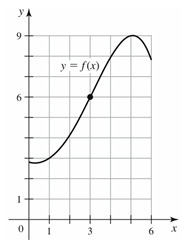
\includegraphics[scale=1.5]{exam1bsec2p7}\end{center}
%\end{comment}

% % % % %
\newpage
\item {\bf (5 pts ea)} When computing derivatives in this problem you must use the limit definitions.  Given the function,
%\[s(t)=\frac{1}{t^2},\]
\[s(t)=\frac{1}{\sqrt{t}}\]
	\begin{enumerate}
	\item write the formula for the slope of the secant line joining the points $(a,s(a))$ and $(b,s(b))$;
	\vspace{14pc}
	
	\item find $s'(1)$;
	\vspace{14pc}
	
	\item write the equation of the line tangent to $s(t)$ at $t=1$.
	\end{enumerate}
	
% % % % %
\newpage
\item {\bf (11 pts ea)} For each function, identify any vertical asymptotes; if there are none, then say so.  Then match the function to its corresponding picture from among the graphs (A)-(C) (see the next page).  
\begin{enumerate}
	\begin{comment}
	\item $f(x)=\frac{x}{x^2+1}$
	\vspace{14pc}
	
	\item $f(x)=\frac{1}{x^2-1}$
	\vspace{15pc}
	
	\item $f(x)=\frac{x}{(x-1)^2}$
	\vspace{15pc}
\end{comment}
%	\begin{comment}	
	\item $f(x)=\frac{x}{x^2-1}$
	\vspace{14pc}
	
	\item $f(x)=\frac{x}{x+1}$
	\vspace{15pc}
	
	\item $f(x)=\frac{1}{(x-1)^2}$
	\vspace{15pc}
%\end{comment}	
\end{enumerate}	
\newpage
\begin{enumerate}[(A)]\centering
\begin{comment}
	\item 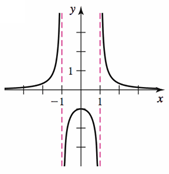
\includegraphics[scale=1.3]{exam1asec2p4B}\hspace{3pc}
	\vspace{3pc}
	
	\item 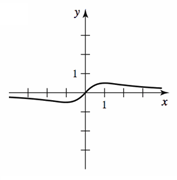
\includegraphics[scale=1.3]{exam1asec2p4A}\hspace{3pc}
	\vspace{3pc}
	
	\item 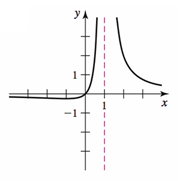
\includegraphics[scale=1.3]{exam1asec2p4C}\hspace{3pc}
	\vspace{3pc}
\end{comment}	
%\begin{comment}
	\item 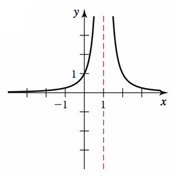
\includegraphics[scale=1.3]{exam1bsec2p4C}\hspace{3pc}
	\vspace{3pc}
	
	\item 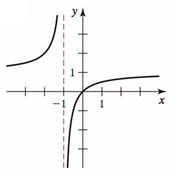
\includegraphics[scale=1.3]{exam1bsec2p4B}\hspace{3pc}
	\vspace{3pc}
	
	\item 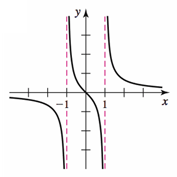
\includegraphics[scale=1.3]{exam1bsec2p4A}\hspace{3pc}
	\vspace{3pc}
%\end{comment}	
\end{enumerate}

% % % % %
%\newpage
%\item {\bf 2.6 P} Determine the interval(s) of continuity for
%\[f(x)=\frac{x^2-4x+3}{x^2-1}\]
%\[f(x)=\frac{x+2}{x^2-4}\]

% % % % %
% % % % %
\newpage
\begin{comment}
\item {\bf (1 pt ea)} Use the graph of $f$ in the figure to find the following values, if they exist.  If a limit does not exist, write ``DNE".

\begin{center}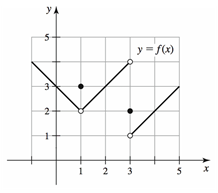
\includegraphics[scale=1.5]{exam1sec2p2}\end{center}

\vspace{1pc}
\begin{multicols}{3}
\begin{enumerate}
	\item $\lim_{x\to 2^-}f(x)$
	\vspace{2pc}
	
	\item $\lim_{x\to 3}f(x)$
	\vspace{2pc}
	
	\item $\lim_{x\to 1^+}f(x)$
	\vspace{2pc}
	
	\item $f(3)$
	\vspace{2pc}
	
	\item $\lim_{x\to 3^-}f(x)$
	\vspace{2pc}
	
	\item $f(1)$
	\vspace{2pc}
	
	\item $\lim_{x\to 2}f(x)$
	\vspace{2pc}
	
	\item $f(2)$
	\vspace{2pc}
	
	\item $\lim_{x\to 1^-}f(x)$	
\end{enumerate}
\end{multicols}
\end{comment}

%\begin{comment}
% % % % %
\newpage
\item {\bf (1 pt ea)} Use the graph of $g$ in the figure to find the following values, if they exist.  If a limit does not exist, explain why.

\begin{center}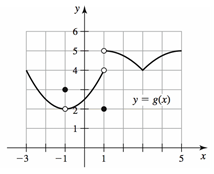
\includegraphics[scale=1.5]{exam1bsec2p2}\end{center}

\vspace{1pc}
\begin{multicols}{3}
\begin{enumerate}
	\item $g(1)$
	\vspace{2pc}
	
	\item $\lim_{x\to -1^+}g(x)$
	\vspace{2pc}
	
	\item $\lim_{x\to 1}g(x)$
	\vspace{2pc}
	
	\item $\lim_{x\to -1^-}g(x)$
	\vspace{2pc}
	
	\item $g(-1)$
	\vspace{2pc}
	
	\item $g(5)$
	\vspace{2pc}
	
	\item $\lim_{x\to -1}g(x)$
	\vspace{2pc}
	
	\item $\lim_{x\to 5^-}g(x)$
	\vspace{2pc}
	
	\item $\lim_{x\to 3}g(x)$	
\end{enumerate}
\end{multicols}
%\end{comment}

% % % % %
\end{enumerate}
\end{document}
